\section{Описание входных и выходных данных}

Входными данными для алгоритма восстановления глубины является путь к существующему в файловой системе изображению
в формате, поддерживаемом OpenCV~\cite{opencv_library}: JPEG, PNG, BMP, TIFF, WebP, PPM, PGM, PBM, SR, RAS.

Результатом работы алгоритма восстановления глубины является нормализованная карта глубин в виде двумерного массива NumPy со значениями в диапазоне [0, 1], где:
\begin{itemize}
    \item темные области (значения ближе к 0) соответствуют объектам, расположенным ближе к камере;
    \item светлые области (значения ближе к 1) соответствуют объектам, расположенным дальше от камеры.
\end{itemize}

Для визуализации результатов используется цветовая схема 'plasma'~\cite{hunter2007matplotlib}, которая обеспечивает интуитивное восприятие глубины сцены.
Пример визуализации представлен на рисунке~\ref{fig:depth_vis}, где показано исходное изображение и предсказанная алгоритмом карта глубин.

% Добавить ссылку на сайт, откуда взяла изображение
\begin{figure}[H]
    \centering
    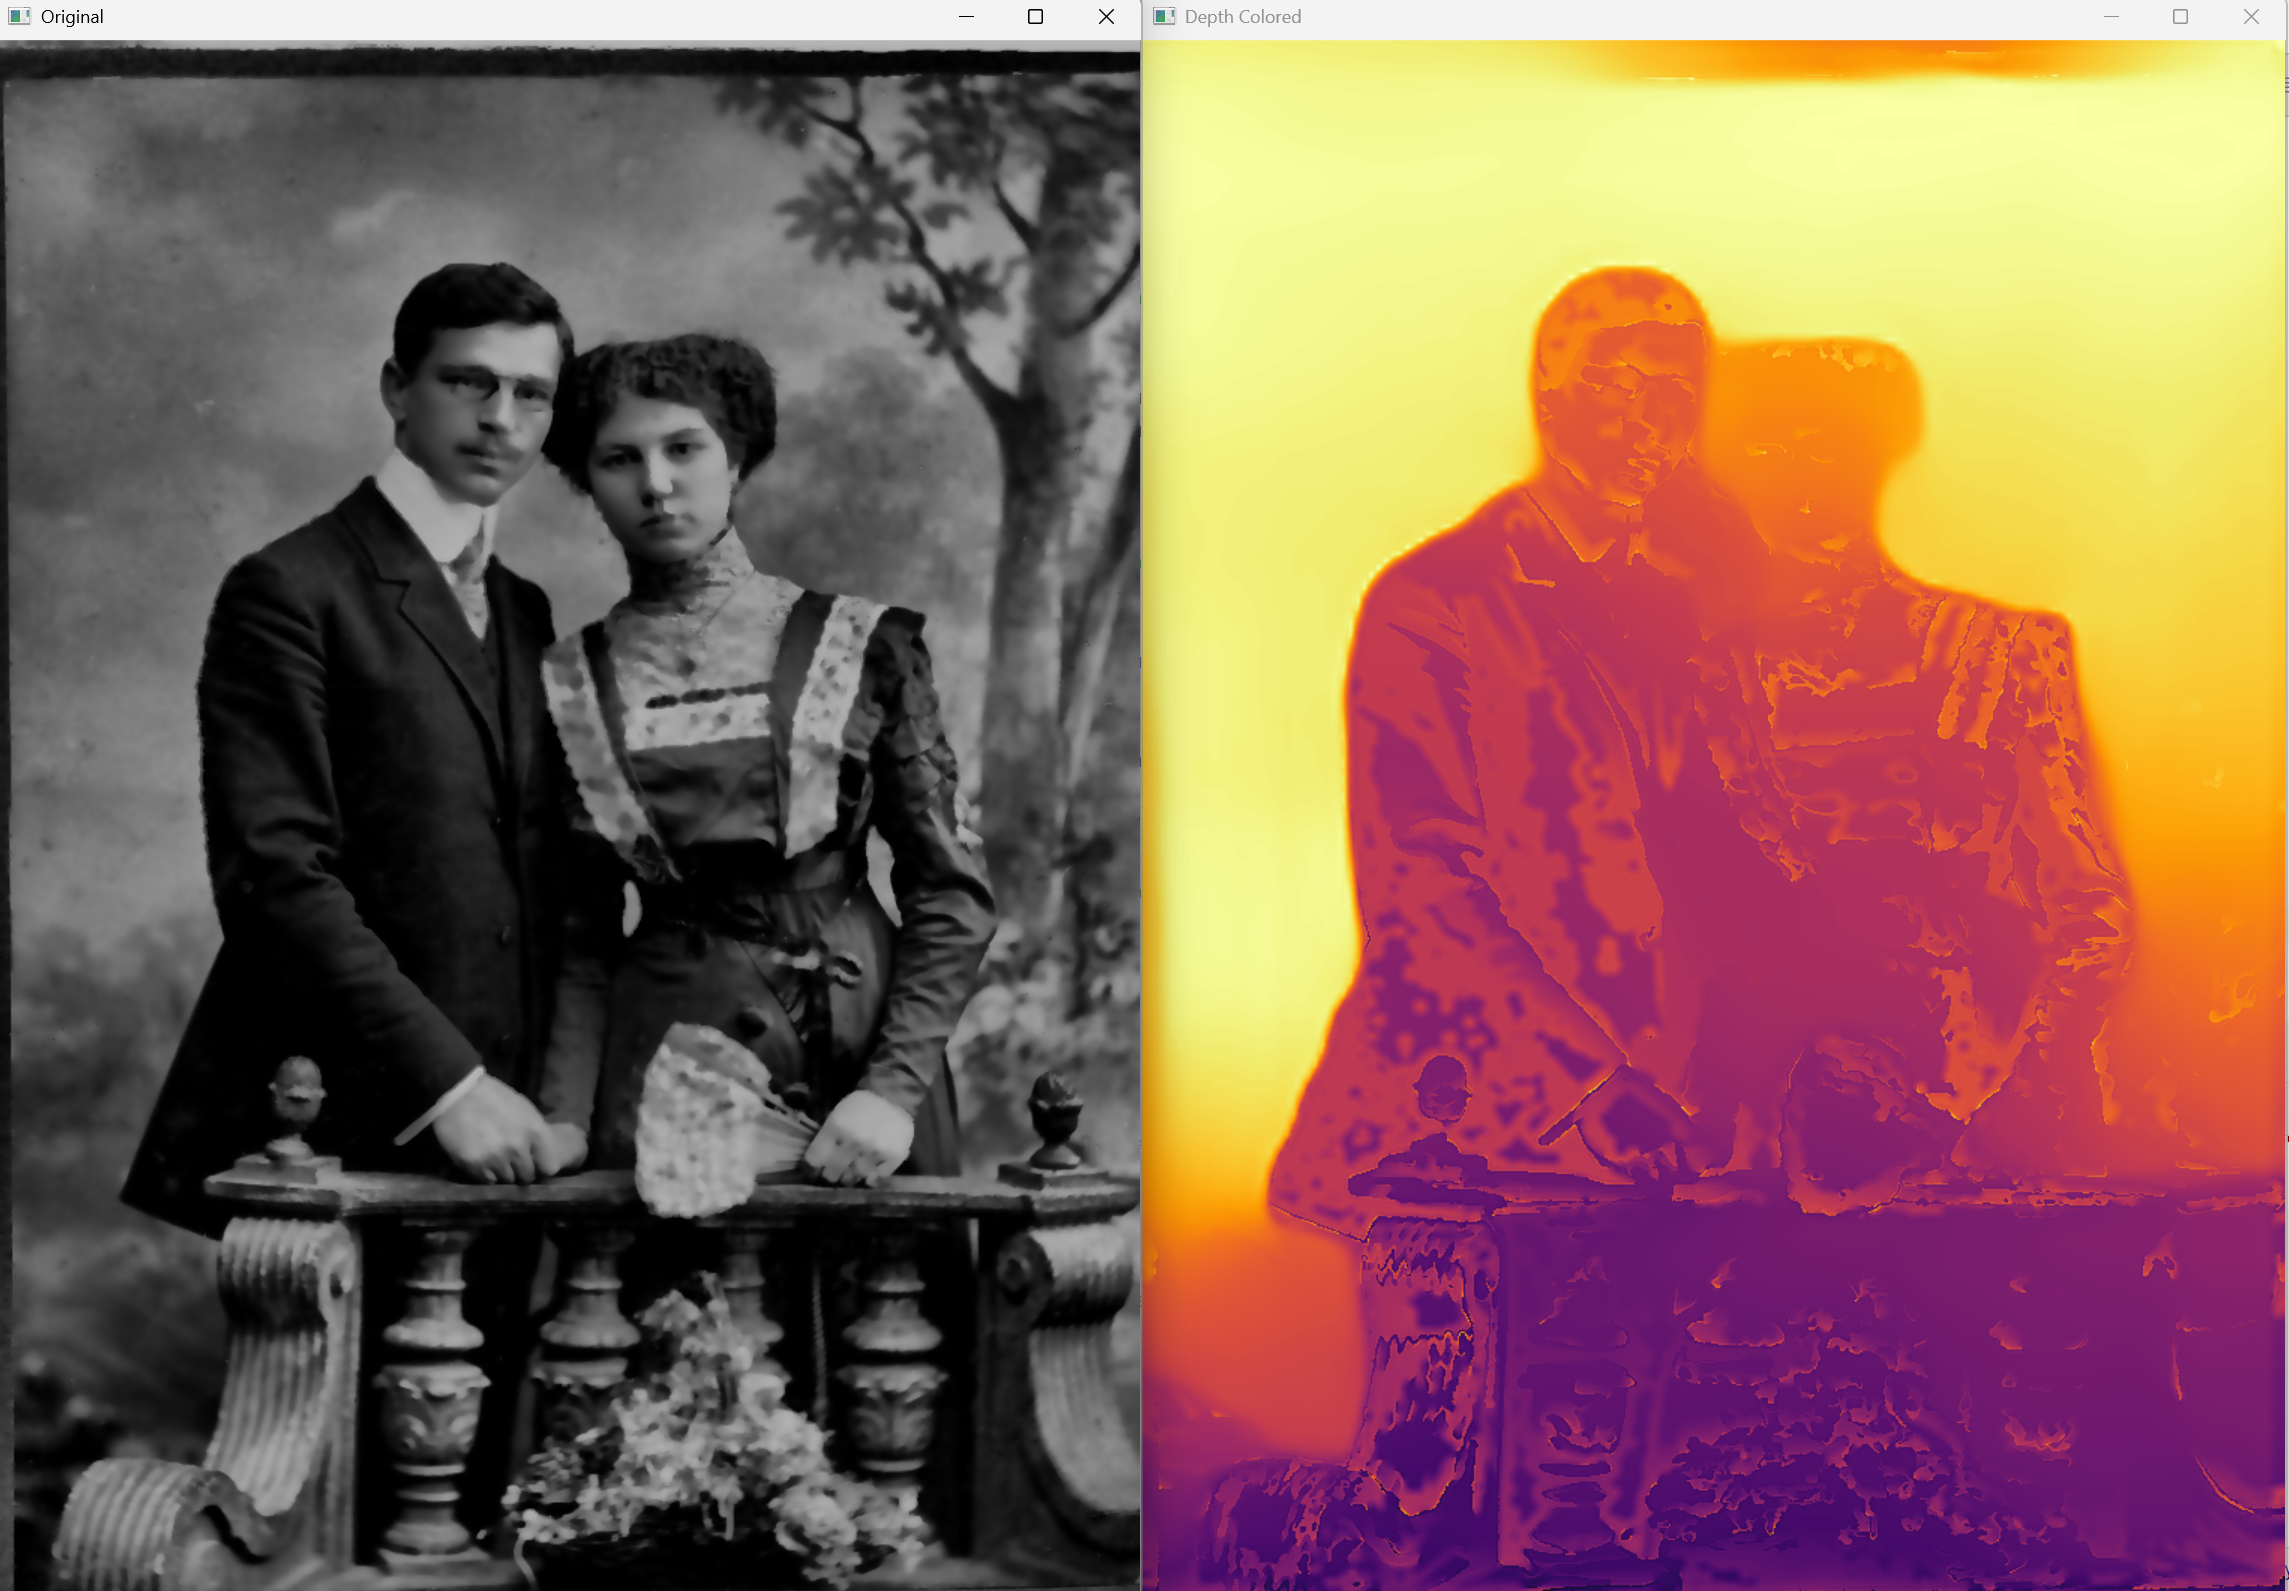
\includegraphics[width=0.9\textwidth]{img/example}
    \caption{Пример визуализации карты глубины: слева -- входное изображение, справа -- предсказанная карта глубин}
    \label{fig:depth_vis}
\end{figure}

\section{Тестирование}

Для обеспечения корректности работы разработанного метода восстановления глубины было проведено модульное тестирование
по методологии "черного ящика" с разделением тестов на классы эквивалентности.

Процесс верификации включает следующие последовательные этапы:
\begin{itemize}
    \item подготовка тестовых изображений, соответствующих каждому классу эквивалентности;
    \item подача на вход метода восстановления глубины пути к тестируемому изображению;
    \item обработка изображения методом восстановления глубины;
    \item визуализация полученной карты глубин в цветовой схеме 'plasma';
    \item сравнение результата с ожидаемым выводом и формирование заключения о корректности.
\end{itemize}

При работе с негативными сценариями дополнительно оценивается корректность обработки исключений,
наличие сообщений об ошибках и соблюдение принципа отказоустойчивости программной системы.
Это гарантирует, что разработанный метод не только правильно функционирует при корректных входных данных,
но и адекватно реагирует на нестандартные ситуации.

В таблице~\ref{tab:test_classes} представлены классы эквивалентности, выделенные для тестирования разработанного метода восстановления глубины из монокулярных изображений.

\begin{table}[H]
    \centering
    \caption{Классы эквивалентности для тестирования}
    \label{tab:test_classes}
    \begin{tabular}{|p{1.5cm}|p{6.5cm}|p{6.5cm}|}
        \hline
        \textbf{Класс} & \textbf{Общее описание} & \textbf{Примеры входных \newline данных} \\
        \hline
        \multicolumn{3}{|l|}{\textbf{Позитивные тесты}} \\
        \hline
        А1 & Обработка черно-белых \newline изображений & Пути к существующим черно-белым изображениям в \newline допустимых форматах (PNG, JPEG) \\
        \hline
        А2 & Обработка изображений в \newline сепии & Пути к существующим \newline изображениям в сепии в \newline допустимых форматах (PNG, JPEG, BMP) \\
        \hline
        А3 & Обработка цветных \newline изображений & Пути к существующим \newline цветным изображениям в \newline допустимых форматах (PNG, JPEG, TIFF) \\
        \hline
        \multicolumn{3}{|l|}{\textbf{Негативные тесты}} \\
        \hline
        Б1 & Обработка отсутствующих файлов & Несуществующие пути к \newline файлам ('/nonexistent.jpg') \\
        \hline
        Б2 & Обработка неподдерживаемых форматов & Пути к файлам с расширениями не из списка допустимых (.txt, .doc) \\
        \hline
        Б3 & Обработка поврежденных изображений & Поврежденные файлы \newline изображений с некорректными данными \\
        \hline
    \end{tabular}
\end{table}

Результаты проведенного тестирования представлены в таблице~\ref{tab:testing_results}.

\begin{table}[H]
    \centering
    \caption{Результаты тестирования метода восстановления глубины}
    \label{tab:testing_results}
    \begin{tabular}{|p{2cm}|p{3.5cm}|p{3.5cm}|p{3.5cm}|p{1.7cm}|}
        \hline
        \textbf{Класс эквив.} & \textbf{Описание входных данных} & \textbf{Ожидаемый результат} & \textbf{Полученный результат} & \textbf{Статус} \\
        \hline
        А1 & Черно-белое изображение в формате JPEG & Успешная загрузка и генерация карты глубины & Карта глубины сгенерирована, сохранена и визуализирована & Пройден \\
        \hline
        А1 & Черно-белое изображение в формате PNG & Успешная загрузка и генерация карты глубины & Карта глубины сгенерирована, сохранена и визуализирована & Пройден \\
        \hline
        А2 & Изображение с эффектом сепии в формате BMP & Успешная загрузка и генерация карты глубины & Карта глубины сгенерирована, сохранена и визуализирована & Пройден \\
        \hline
        А3 & Цветное изображение размером 4K (3840×2160) & Успешная обработка с автоматическим масштабированием & Изображение масштабировано и обработано корректно & Пройден \\
        \hline
        Б1 & Путь к несуществующему файлу ('/nonexistent.jpg') & Сообщение об ошибке с указанием на отсутствие файла & "Ошибка: файл '/nonexistent.jpg' не существует" & Пройден \\
        \hline
        Б2 & Путь к файлу с расширением .txt & Сообщение о неподдерживаемом формате файла & "Ошибка: формат '.txt' не поддерживается" & Пройден \\
        \hline
        Б3 & Поврежденный JPEG-файл & Сообщение о невозможности декодирования изображения & "Ошибка при декодировании изображения" & Пройден \\
        \hline
    \end{tabular}
\end{table}

Проведенное тестирование показало, что разработанный метод корректно обрабатывает изображения различных поддерживаемых форматов,
а также адекватно реагирует на некорректные входные данные, предоставляя пользователю информативные сообщения об ошибках.

\section{Вывод}
В технологическом разделе выполнена полная программная реализация гибридного метода восстановления глубины из монокулярных изображений.

Для решения поставленной задачи был выбран язык Python с экосистемой специализированных библиотек (OpenCV, PyTorch, NumPy и др.),
что обеспечило эффективную работу с изображениями, применение моделей машинного обучения и визуализацию трехмерных данных.

Разработанный алгоритм успешно прошел тестирование на различных типах изображений (цветных, черно-белых, с эффектом сепии)
и продемонстрировал корректную обработку исключительных ситуаций, что подтверждает работоспособность созданного решения.

